\subsubsection{Cadre Général}

Pour chaque environnement annoté, le module de raisonnement effectue une mise à jour des probabilités d'apparition d'une annotation en fonction d'une forme.

\[ P(Annotation|Forme) = \frac{P(Forme|Annotation) \times P(Annotation)}{P(Forme)} \]

\paragraph{Exemple de la figure~\ref{img_annotations}}
Imaginons que nous souhaitons entraîner \cogito{} à identifier des formes géométriques basiques : \emph{rond}, \emph{carré}, \emph{croix} et \emph{triangle}. Admettons que notre IA soit capable de reconnaître dans son environnement les formes correspondantes mais qu'elle ne sache pas les associer aux annotations correspondantes.

\begin{figure}[H] 
\centering
    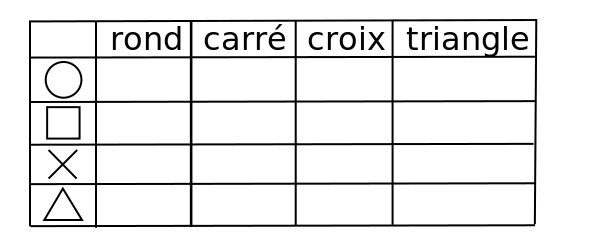
\includegraphics[width=0.5\textwidth]{files/raisonneur/annotations} 
\caption{Association formes-annotations.} 
\label{img_annotations}
\end{figure}

Partant de cet état initial, l'IA doit apprendre de ses expériences. Pour ce faire elle doit mettre à jour les probabilités qu'une annotation soit rattachée à un environnement pour chaque nouvel environnement rencontré. La figure~\ref{img_annotations_1} met en évidence les probabilités calculées suite à la rencontre d'un environnement présentant la forme \emph{rond}.

\begin{figure}[H] 
\centering
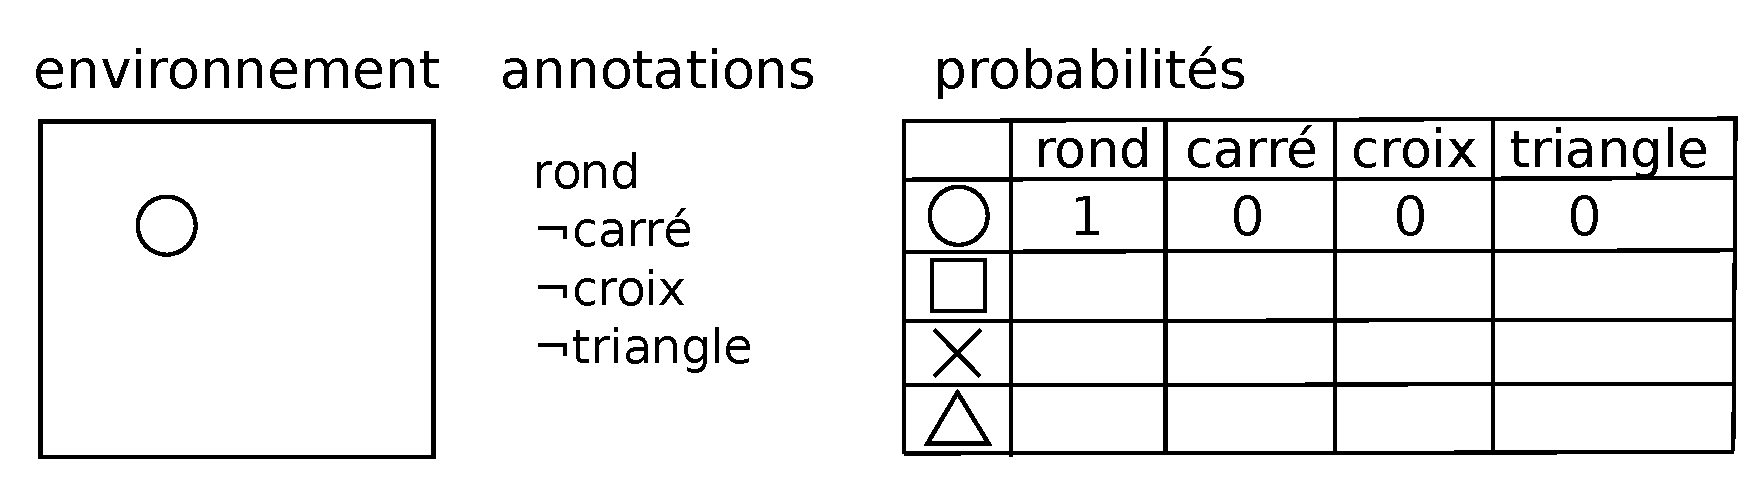
\includegraphics[width=\textwidth]{files/raisonneur/annotations_1} 
\caption{Association formes-annotations basique à l'étape 1.} 
\label{img_annotations_1}
\end{figure}

Le calcul des probabilités s'effectue de la même manière pour un environnement qui présente un ensemble de formes, comme illustré sur la figure~\ref{img_annotations_2}. Il existe alors une ambiguïté car le système ne peut pas savoir quelle forme est responsable de quelle annotation.  

\begin{figure}[H] 
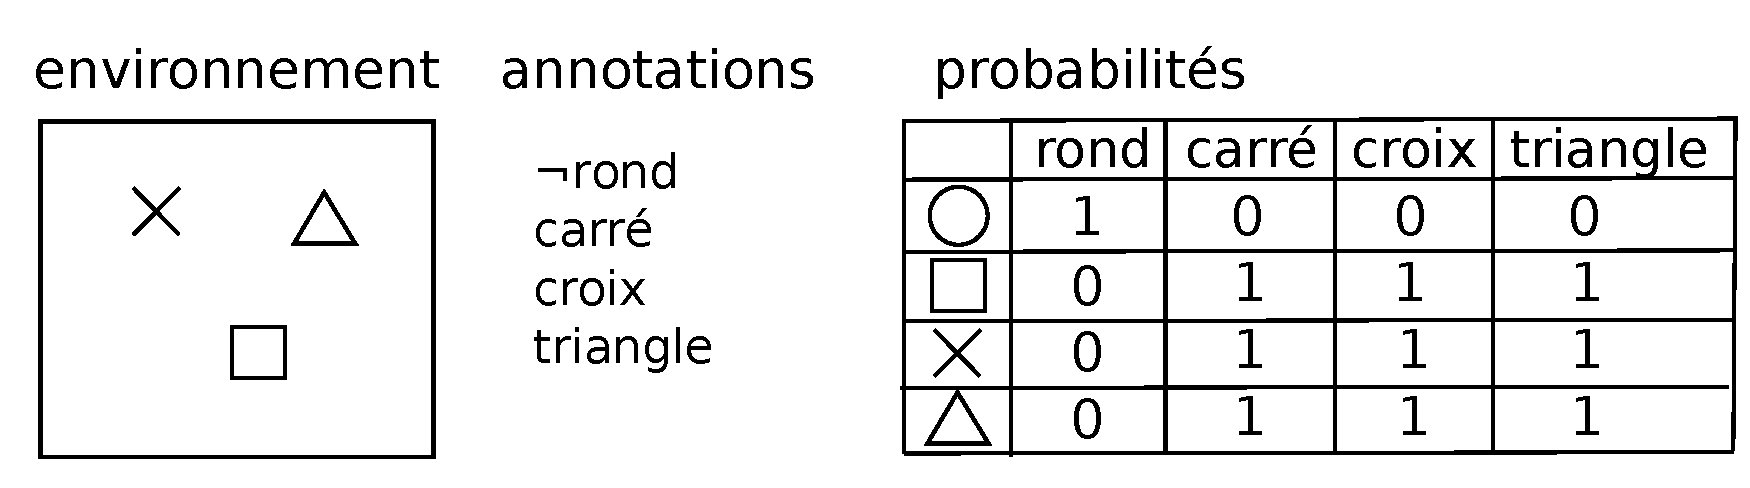
\includegraphics[width=\textwidth]{files/raisonneur/annotations_2} 
\caption{Association formes-annotations multiple à l'étape 2.} 
\label{img_annotations_2}
\end{figure}

Cependant, cette ambiguïté est levée par l'expérience qui confrontera le système avec des ensembles variés de formes. Par conséquent, seul l'annotation correcte pour chaque forme conserve une probabilité certaine comme il est possible de l'observer sur les figures \ref{img_annotations_3}, \ref{img_annotations_4} et \ref{img_annotations_5} illustrant l'évolution du système. 

\begin{figure}[H] 
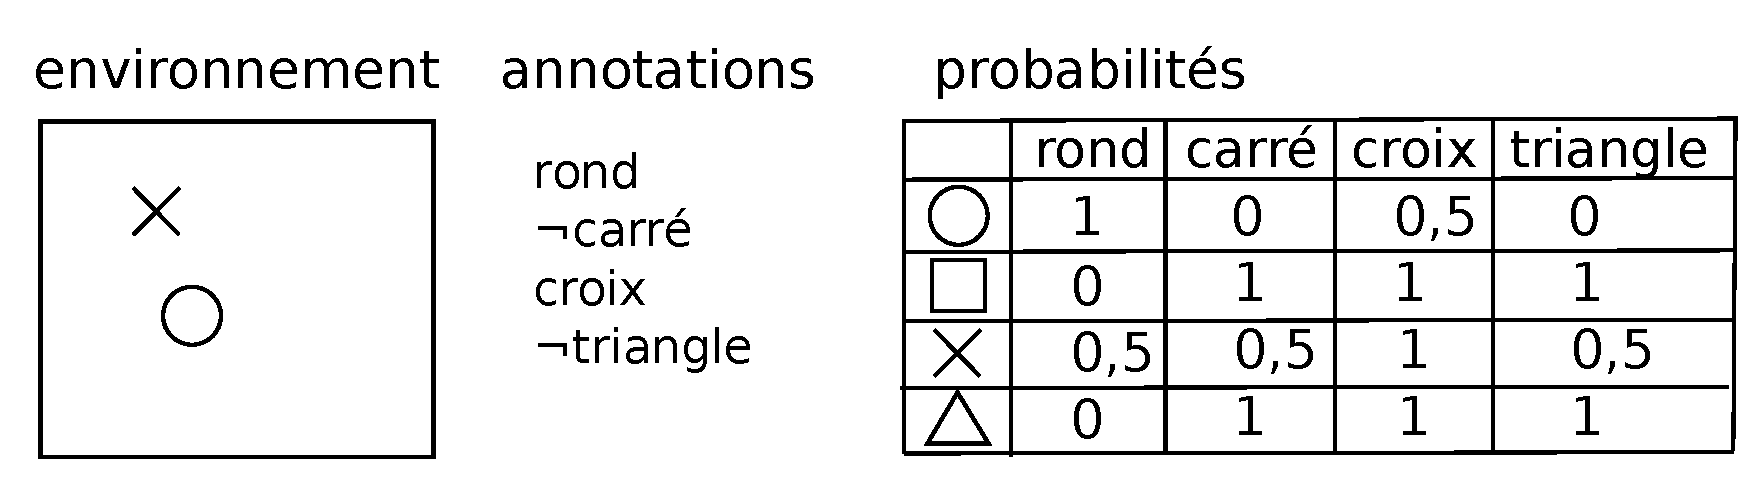
\includegraphics[width=\textwidth]{files/raisonneur/annotations_3} 
\caption{Association formes-annotations à l'étape 3.} 
\label{img_annotations_3}
\end{figure}

\begin{figure}[H] 
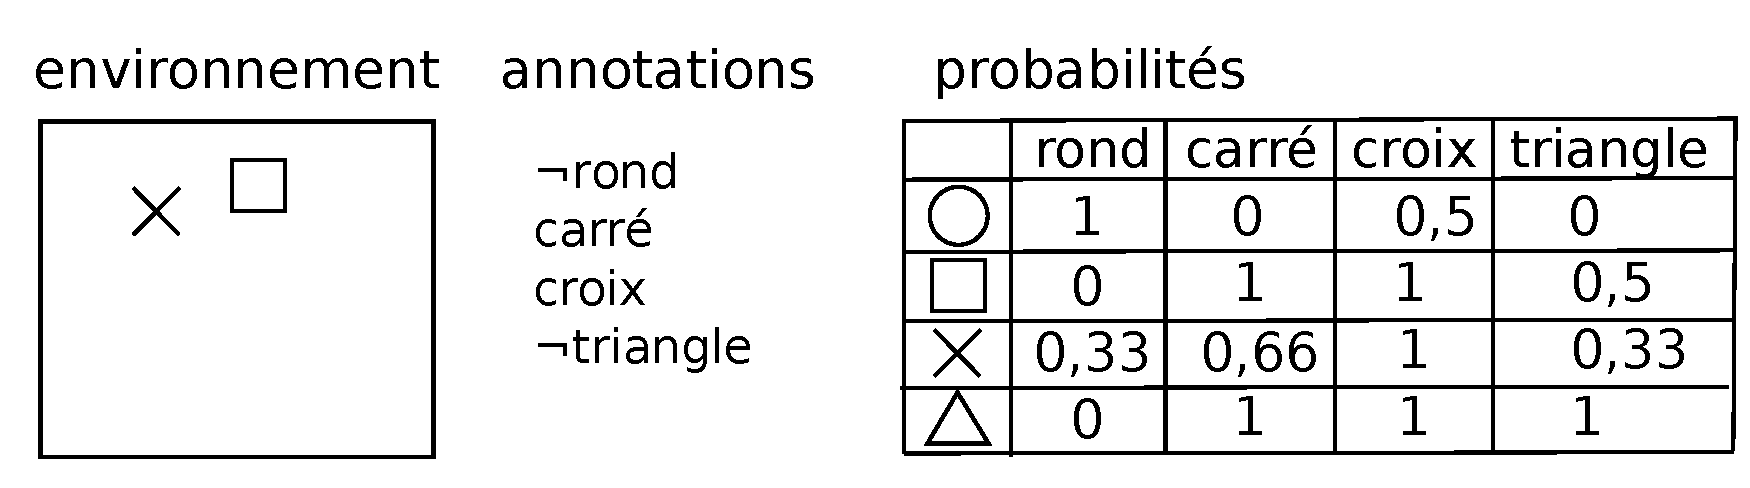
\includegraphics[width=\textwidth]{files/raisonneur/annotations_4} 
\caption{Association formes-annotations à l'étape 4.} 
\label{img_annotations_4}
\end{figure}

\begin{figure}[H] 
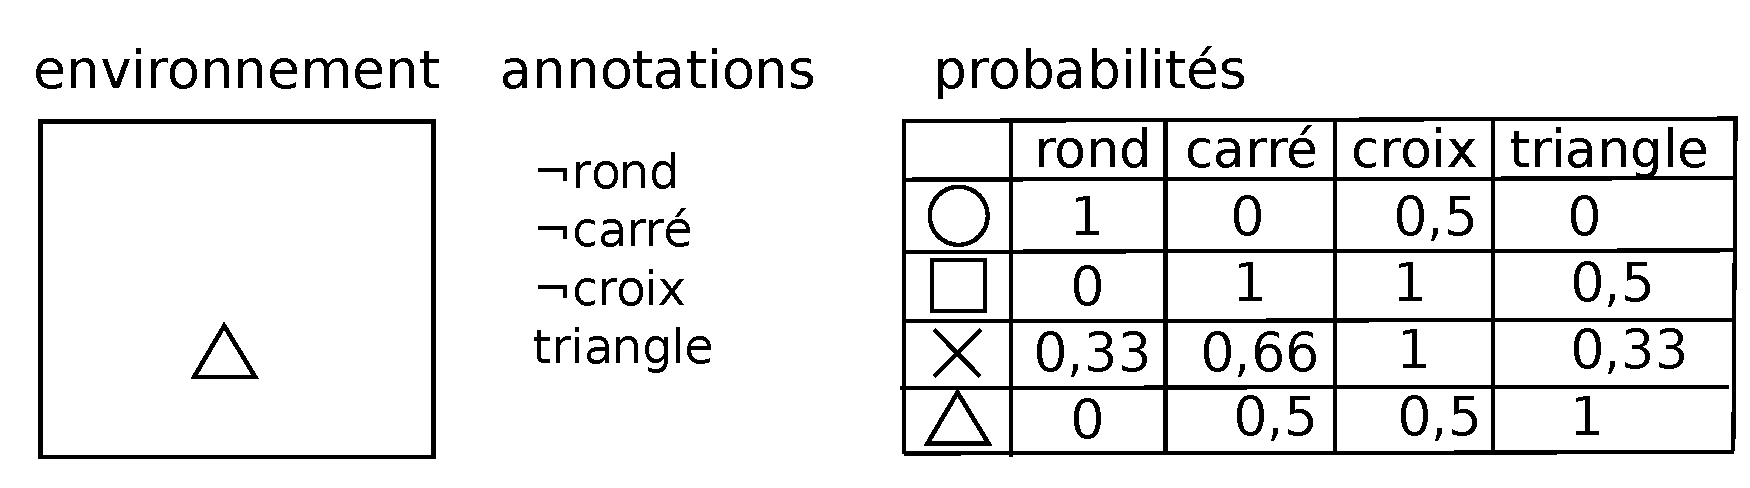
\includegraphics[width=\textwidth]{files/raisonneur/annotations_5} 
\caption{Association formes-annotations à l'étape 5.} 
\label{img_annotations_5}
\end{figure}

Il est important de noter que la certitude, représentée par une probabilité égale à $1$, ne peut être garanti que si les annotations fournies au système lors de sa période d'apprentissage sont exemptes d'erreurs. Cependant, une erreur d'annotations lors de l'apprentissage certes diminuerai la probabilité associé à l'annotation correct mais pour vu que le jeux d'apprentissage soit assez grands, celle-ci resterai la plus probable.

\subsubsection{Application aux jeux de plateau}

Dans le cadre des jeux de plateau deux annotations sont fournies :
\begin{itemize}
\item \emph{victoire},
\item \emph{défaite}.
\end{itemize}
Il est évident, mais nécessaire, de préciser que :
\begin{itemize}
\item \emph{victoire} $\rightarrow{}\neg{}$ \emph{défaite}
\item \emph{défaite} $\rightarrow{}\neg{}$ \emph{victoire}
\end{itemize}

Ces annotations doivent être fournies directement par l'environnement sans intervention humaine, nous sommes donc sûr de l'apprentissage par renforcement.
